% !TEX encoding = UTF-8 Unicode
\chapter*{Conclusion}           % ne pas numéroter
\label{chap-conclusion}         % étiquette pour renvois
\phantomsection\addcontentsline{toc}{chapter}{\nameref{chap-conclusion}} % inclure dans TdM

Effective control of grinding circuits is challenging for a number of reasons. This work focussed on the problem of variations in the ore feed properties to the \gls{SAG} mill, which \hlep{are believed to have} a \hlep{significant} impact on grinding process control and performance. \hljb{Timely detection and estimation of ore disturbances in real time could potentially allow a process control system to reduce variations in key process variables, leading to benefits such as increased throughput and more consistent product quality.}

Traditional control design methods utilise stochastic disturbance models based on the assumption of Gaussian noise. However, there is evidence that real ore disturbances in mining operations exhibit complex dynamic behaviour, such as abrupt step changes and ramps. \hljb{The objectives of the research were to identify a suitable model for representing typical disturbances in grinding operations and to propose an observer framework utilizing the model.} The randomly-occurring deterministic disturbance (\gls{RODD}) model defined by \cite{macgregor_duality_1984} is an alternative to the standard disturbance model, capable of representing a range of realistic disturbances that are common in industrial process operations, including step changes and ramps. Standard state estimators such as the Kalman filter, used to filter process measurements in control applications, are \hlep{not ideal} when there are \gls{RODD}s. One solution to this problem is the sub-optimal multiple-model observer approach. \hljb{The main contribution of this work was to identify and evaluate the performance of two types of multiple-model observer specifically designed for {\gls{RODD}} estimation.}

Three simulation experiments were carried out to evaluate the performance of the observers. In the first two experiments, simple linear process models were used, one with a single \gls{RODD} input and a single process output, the second with two \gls{RODD}s and two output measurements. In the third experiment, a realistic grinding process simulation model by \cite{perez_garcia_dynamic_2020} was used. To produce a realistic disturbance, an ore feed was simulated that randomly and abruptly switched between two ore mixtures with different particle size distributions.

In each experiment, a simulated measurement noise was added to the process outputs and the performance of the multiple-model observers was compared to a standard Kalman filter by calculating the root-mean-squared errors (\gls{RMSE}) between the observer estimates and the true (simulated) process outputs. \hl{The performance of each of the multiple model algorithms was found to be quite similar. However, the performance improvement of the multiple model observers relative to a Kalman filter was significant, although the relative improvement was} different in each experiment. In the first experiment a significant reduction in estimation errors of 36\% was demonstrated. In the second experiment, the reduction was not as large but still significant. In the third experiment on the grinding process model, the estimation errors of the multiple model observers were only 6-8\% lower than the Kalman filter. This variation in the performance advantage was attributed to specific characteristics of the systems simulated, indicating that the benefits of the multiple model observers are dependent on the type of system they are applied to.

However, further analysis showed that the multiple-model observers had a significant advantage in steady-state periods (between ore changes) when they were significantly less sensitive to the measurement noise. Sensitivity to measurement noise can be a serious problem in process control systems, therefore this could justify the added complexity of these observers. A sensitivity analysis also showed that the performance of the observers was less sensitive to parameter settings than that of a Kalman filter, indicating that the risk of a significant deterioration in performance if the system changed\hl{, or if the model parameters were not estimated correctly,} is low.

\section*{Limitations}

It is important to note the main limitations of this work. Firstly, although the multiple model observers offer a clear improvement in terms of lower estimation errors compared to a standard Kalman filter, how these results translate into benefits in terms of improved process control was not investigated. Secondly, the simulations used to evaluate the observers did not include any disturbances other than one or two RODDs. In real grinding operations, there are many sources of disturbances in addition to changes in the ore particle size. There is no guarantee that the observers will perform as well in more complex operating conditions such as those experienced in real operations. Thirdly, due to a lack of good data on real ore disturbances, it is not known whether the parameters of the simulated ore disturbance used in the third experiment are realistic or representative of typical ore disturbances. The simple switching behaviour was chosen mainly to aid the evaluation process. Fourth, the original implementation of the multiple model algorithm based on sequence pruning \citep{eriksson_classification_1996} included a feature to adapt online to the measurement noise level. This feature was not implemented in this work. Although the measurement noise level was constant in the simulations, there is a possibility that this feature could improve the performance of this algorithm.

Finally, the grinding process simulation model has many limitations. Although it is based on phenomenological models of the process and was calibrated to data from a real operation, it is unlikely to capture all the important dynamics, complex behaviour, and internal states of a real operation. It is therefore a simplification of reality and results demonstrated on the simulation model are not guaranteed to be achievable in a real operation.

\section*{Future research} \label{sec:future-research}

A number of opportunities were identified during the course of this work that are potentially worth pursuing. These may be organised into three categories: (i) additional simulations to further evaluate the multiple-model observers and quantify potential benefits, (ii) investigation of other disturbance models and methods of identifying their parameters using data from real operations, and (iii) investigation of methods of state estimation for non-Gaussian disturbance processes.

In the first category, the obvious next step is to simulate the multiple-model observers in closed-loop with a controller. The grinding process simulation model has a number of manipulated variables and output measurements that could be utilised in a multi-input, multi-output (\gls{MIMO}) control scenario. The diagram in Figure \ref{fig:grind_sim_io_diag} illustrates one possible configuration that could be simulated. There are three manipulated input variables, one unmeasured ore disturbance, and four measured output variables (not all the output variables are controllable with the available inputs so some may be used solely for state estimation or simply constrained within a range).
\begin{figure}[ht]
	\centering
	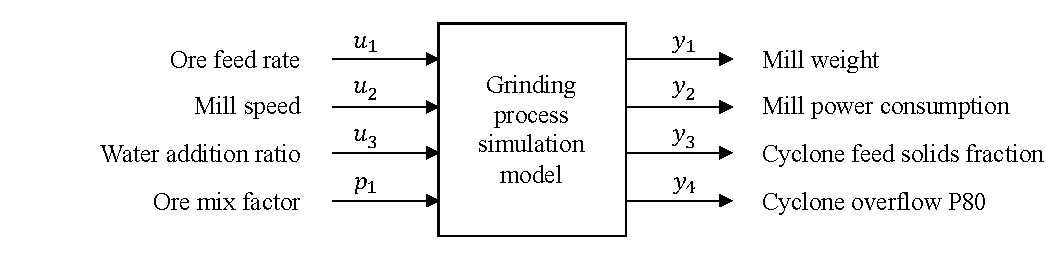
\includegraphics[width=15cm]{images/grind_sim_io_diag.pdf}
	\caption{\hlad{Possible MIMO model for evaluating grinding process control performance}}
	\label{fig:grind_sim_io_diag}
\end{figure}
\hlad{Some of these process variables, such as mill weight, power consumption, and slurry density (i.e. solids fraction), are likely to yield more timely and reliable information for estimation of ore disturbances than the product particle size, which was the only measurement used in this work. Not only are these variables located physically closer to the disturbance input, they are typically sampled at higher rates and more accurately than the product particle size, which requires an online analyser. This is interesting, because the simulations in this work indicated that the multiple-model observers offered a superior advantage to a Kalman filter when the signal-to-noise ratio was higher. Another objective in simulating MIMO control schemes, should be to investigate the potential to utilize improved state estimates to reject the effects of the disturbance on key process variables, such as product particle size.}

For the MIMO simulations, a model-predictive controller (\gls{MPC}), which requires a full set of state estimates, would be a good choice \hl{since it allows input and output constraints to be handled. For example, maximum power consumption limits grinding throughput and quality in most operations.} As in this work, the goal of these simulations would be to determine the controller performance when simulated with a multiple-model observer compared to simulations with a Kalman filter. Various metrics, \hl{in addition to those used in this work,} could be used, such as the \gls{RMSE} between the controlled variables and the set-points \hl{(i.e. tracking error)}. \hlad{It is also important to test the ability of the observers to simultaneously estimate multiple disturbances in addition to the {\gls{RODD}}. Since there are many sources of disturbances in real operations, it is critical that the multiple-model observers can perform well under realistic conditions}. Further work should also evaluate the observers with other types of \gls{RODD}, such as the ramp \eqref{eq:RODD-ramp} and the combined steps-and-ramps \gls{RODD} \eqref{eq:RODD-step-ramp}.

In the second category, the hidden Markov model (\gls{HMM}) approach described by \cite{wong_realistic_2009} is a natural extension of the \gls{RODD} worth considering. Also, the bounded random walk (\gls{BRW}) described in Section \ref{sec:bounded} could be useful for simulating realistic disturbances. It may be possible to extend the basic idea of the \gls{BRW} to \gls{RODD}s. One simple way is to simulate two \gls{BRW}s in parallel and simply switch between them randomly. This could be useful for representing switching ore streams coming from different parts of a mining operation. An interesting question that could be explored, is whether a bounded \gls{RODD} is easier or more difficult to estimate than an unbounded \gls{RODD}. In the case of a bounded \gls{RODD}, the possible directions and magnitudes of shocks are constrained, as they would be in a real operation. If this model can be incorporated into a process observer, it could hypothetically perform better than an observer based on the standard \gls{RODD} model.

There are two important challenges that need to be overcome to make progress on realistic disturbance modelling. Firstly, the need for good data on actual disturbances. Ore properties are generally difficult to measure at a frequency high enough to identify the dynamic nature of the variability. However, various online particle size analysers based on imaging technology are now in use in some operations (see \cite{steyn_investigating_2018} for example). Although these do not provide a true measure of the particle size distribution they should provide valuable insight into the dynamic nature of the variations, which is more important for evaluating control systems. 

The second challenge, as mentioned in Section \ref{sec:sys-id}, is the problem of identifying disturbance models from data. This is difficult because \gls{RODD}s are hybrid dynamical systems with unknown discrete states \citep{sworder_boyd_1999}. Various developments in the field of non-linear system identification may be applicable. For example, \cite{schon_sequential_2015} describe the family of techniques known as \textit{sequential Monte Carlo} (\gls{SMC}) methods, which are able to identify system models with non-Gaussian disturbances. Before attempting to estimate models based on real data it makes sense to evaluate potential methods on simulated data. \cite{wong_realistic_2009} described the difficulties they encountered estimating a variety of \gls{HMM} models from simulated data.

Finally, when it comes to state estimation for non-Gaussian random processes, the solution should follow naturally from solving the system identification problem. \gls{SMC} methods necessarily solve the joint problems of parameter estimation and state estimation simultaneously, so the problem of online state estimation is simply the online application of \gls{SMC}.

Developing practical methods of identifying and simulating realistic industrial disturbances could have many potential benefits in control system design and implementation, especially in the mineral processing industry where unmeasured disturbances are one of the main challenges for process control. At the simplest level, more realistic simulations of disturbances will allow process control systems to be more comprehensively tested and evaluated for potential application. However, beyond this immediate goal, incorporation of disturbance models based on the characteristics of the actual disturbances into process observers, as in this work, and potentially into control algorithms, could lead to the development of more advanced control systems that exceed the performance of standard techniques in these applications.
